%======================================================================
\chapter{Motivating Example}
%======================================================================

We present a motivating example to showcase how a newly added unchecked exception can cause a \gls{bbc} in the client code. We select the client/library pair from the DUETS dataset~\cite{durieux21:_duets}. We also demonstrate how we wrote a test case to verify the behavioural breaking change in the client caused by the updated library.

For this motivating example, we use \texttt{HttpAsyncClientUtils}\footnote{\url{https://github.com/iiweniiang/HttpAsyncClientUtils}} as our client. This client appears in the DUETS dataset. It declares version 4.4.6 of the \texttt{httpcore} library as one of its dependencies. Since the release of version 4.4.6, the developers of the \texttt{httpcore} library have released several newer versions. The latest available version is 4.4.16.\footnote{While \texttt{httpcore} 5.2.4 is in fact the latest version of this library, the library developers have released \texttt{httpcore5} as a distinct Maven component from \texttt{httpcore4}, and labelled \texttt{httpcore}(4) as end-of-life.}.

The update from version 4.4.6 to 4.4.16 of the \texttt{httpcore} library introduces a check for a new condition. In this update, the library checks the length of the argument provided by the client to the \gls{api}. Version 4.4.16 verifies whether the argument length is equal to "0", and if so, throws a new \texttt{IllegalArgumentException}. In the specific case of \texttt{HttpAsyncClientUtils} as the client and \texttt{httpcore} as the library, the client uses the \gls{api} method that includes this newly added check. We now demonstrate how UnCheckGuard identifies that the client is using a method from the library, detects the newly added exception, and verifies that the exception is actually triggerable by the client in order to avoid false positives.

\section{Detecting invocation of a library method in client}

A newly added unchecked exception in a library is only relevant to a client if the client actually uses the library method that introduces the exception. UnCheckGuard eliminates analysis of unused library methods by first analyzing the client for external method invocations. We perform this analysis by identifying all external method calls within the client code using Sootup~\cite{Karakaya24:_sootup}. In the case of \texttt{HttpAsyncClientUtils} as the client, it calls the \texttt{HttpCore} library from its public \texttt{createAsyncClient(boolean)}\footnote{Fully-qualified: method \texttt{createAsyncClient(boolean)} returning a \texttt{CloseableHttpAsyncClient} on class \texttt{Util.HttpClientUtil.HttpAsyncClient}.} method, which creates an \texttt{HttpHost} with an empty \texttt{host}. This method accepts a \texttt{proxy} parameter and includes the following code:

\begin{lstlisting}[language=Java]
 if (proxy) {
  return HttpAsyncClients.custom()
   .setConnectionManager(conMgr)
   .setDefaultCredentialsProvider(credentialsProvider)
   .setDefaultAuthSchemeRegistry(authSchemeRegistry)
   .setProxy(new HttpHost(host, port))
   .setDefaultCookieStore(new BasicCookieStore())
   .setDefaultRequestConfig(requestConfig).build();
 } else {
   // ...
\end{lstlisting}

The \texttt{HttpAsyncClientUtils} client declares the two variable (host and port) required for \texttt{HttpHost} (line 6 in the above code) in the following way:
\begin{lstlisting}[language=Java]
    private String host = "";
    private int port = 0;
   // ...
\end{lstlisting}

The client initializes \texttt{host}, a private field of type \texttt{String}, as an empty string and sets \texttt{port} to 0. As a result, the client calls \texttt{<init>(String, int)}\footnote{Specifically, constructor \texttt{<init>(String, int)} returning a \texttt{void} on class \texttt{org.apache.http.HttpHost}} with the host set to an empty string and the port set to 0.
% Thus, calling \texttt{createAsyncClient(true)} triggers an exception when executed with
% \texttt{httpcore} version 4.4.16 but not with 4.4.6.

After collecting all external method calls made by the client \texttt{HttpAsyncClientUtils}, UnCheckGuard begins comparing the version of the library currently used by the client with the latest available version. It stores all external method invocations made by the client—not just those to the \texttt{HttpHost} library in a \texttt{JSON} file. If UnCheckGuard detects a newly added exception in any of these external method calls, it then uses taint analysis to check whether the exception is actually reachable from the client. For this client, UnCheckGuard identifies a call to \texttt{HttpHost}. The next step for UnCheckGuard is to detect the newly added exception and verify its reachability.


% To detect that our \texttt{HttpAsyncClientUtils} client calls a method from \texttt{httpcore-4.4.6} which, upon upgrading to \texttt{httpcore-4.4.16}, may throw a new unchecked exception, UnCheckGuard begins by identifying all external library methods invoked anywhere in the client. It then analyzes both the current and the latest versions of the library to determine whether any newly introduced unchecked exceptions are reachable from the client's code. Here, reachability means that the client can trigger the exception in the library on some execution of the program, using values it passes to the library as parameters.

\section{Detecting newly added exception in Library} 

UnCheckGuard in the previous step found that the client \texttt{HttpAsyncClientUtils} makes a call to the constructors for the \texttt{org.apache.http.HttpHost} class. UnCheckGuard now analyzes the set of exceptions thrown by the constructor for both 4.4.6 and 4.4.16 version.

% To detect this change, UnCheckGuard processes JAR files for both \texttt{httpcore-4.4.6} and \texttt{httpcore-4.4.16}. It uses SootUp~\cite{Karakaya24:_sootup} to construct a call graph using Class Hierarchy Analysis (CHA) starting from the public \texttt{<init>(String, int)}\footnote{Specifically, constructor \texttt{<init>(String, int)} returning a \texttt{void} on class \texttt{org.apache.http.HttpHost}} constructor on \texttt{HttpHost} and identifies the set of all methods transitively reachable by the client (which we will discuss below). UnCheckGuard then collects all unchecked exceptions thrown within this set of reachable methods, for both library versions.
To determine whether the newer version of the library introduces a newly added exception, UnCheckGuard analyzes the JAR files for \texttt{httpcore-4.4.6} and \texttt{httpcore-4.4.16}. It performs this analysis using SootUp~\cite{Karakaya24:_sootup}. UnCheckGuard constructs a call graph using Class Hierarchy Analysis (CHA), starting from the public \texttt{<init>(String, int)} constructor in \texttt{HttpHost}. With the help of this call graph, UnCheckGuard identifies the set of all methods transitively reachable by the client (discussed below). It then collects the list of exceptions present within those methods. UnCheckGuard performs this process for both the currently used version of the library and the newer version. During this step, it stores the list of exceptions found in different methods of a particular \gls{api} in a \texttt{JSON} file, as this information is needed later for comparison.

Now, based on the call graph constructed for the public \texttt{<init>(String, int)} constructor on \texttt{HttpHost}, UnCheckGuard find that the constructor calls the static method \texttt{Args.containsNoBlanks()}\footnote{Fully-qualified name: method \texttt{containsNoBlanks(java.lang.CharSequence,java.lang.String)} returning a \texttt{java.lang.CharSequence} on class \texttt{org.apache.http.util.Args} } in the version 4.4.16.

% All constructors for the \texttt{org.apache.http.HttpHost} class transitively call
% the static method \texttt{Args.containsNoBlanks()}. Between version 4.4.6 and version 4.4.16, the \texttt{httpcore}
% developers added the following lines of code to \texttt{containsNoBlanks()}:

Upon a manual inspection of the static method \texttt{Args.containsNoBlanks()}, we find that the developers have added the following lines of code to the 4.4.16 version:

\begin{lstlisting}[language=Java]
  public static <T extends CharSequence> T containsNoBlanks(final T argument, final String name) {
        ...
        if (argument.length() == 0) {
            throw new IllegalArgumentException(name + " may not be empty");
        }
        ...
        return argument;
    }
\end{lstlisting}

Specifically, all \texttt{HttpHost} constructors take a \texttt{hostname} parameter and call \texttt{containsNoBlanks()}
with that parameter (to check that it contains no blanks). In the case when the length of the argument (\texttt{host}) is equal to zero it throws a unchecked exception \texttt{IllegalArgumentException}. A client can therefore trigger this newly added exception
in a client by attempting to instantiate a new \texttt{HttpHost} object and passing it an empty
\texttt{hostname}.

\begin{figure}[htbp]
    \centering
    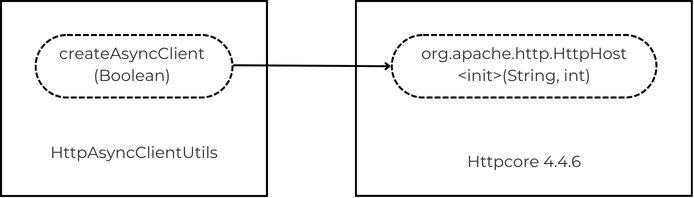
\includegraphics[width=0.6\textwidth]{diagram/httpcore6.png}
    \caption{External method call from \texttt{createAsyncClient(Boolean)} in \texttt{HttpAsyncClientUtils} to the \texttt{HttpHost} constructor \texttt{<init>(String, int)} in \texttt{Httpcore 4.4.6}.}
    \label{fig:httpcore6}
\end{figure}

\begin{figure}[htbp]
    \centering
    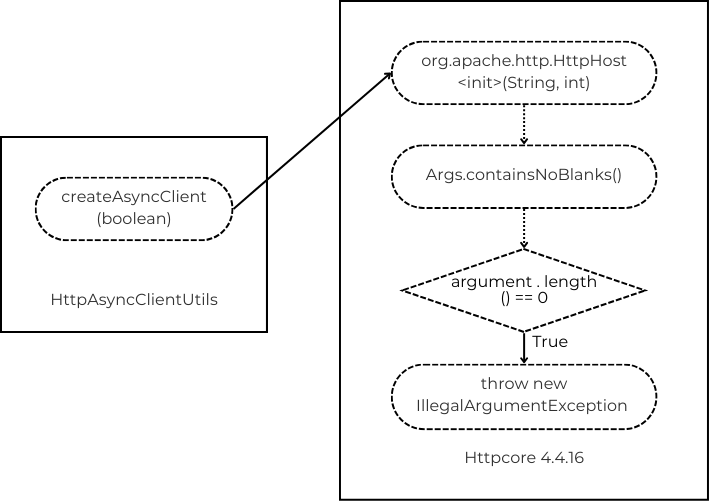
\includegraphics[width=0.75\textwidth]{diagram/httpcore16.png}
    \caption{External method call from \texttt{createAsyncClient(Boolean)} in \texttt{HttpAsyncClientUtils} to the \texttt{HttpHost} constructor \texttt{<init>(String, int)} in \texttt{Httpcore 4.4.16}, which internally validates arguments using \texttt{Args.containsNoBlanks()} and may throw an \texttt{IllegalArgumentException}.}
    \label{fig:httpcore16}
\end{figure}

Our UnCheckGuard tool analyzes the changes in \texttt{httpcore} and finds that, in version 4.4.16, all of the \texttt{HttpHost} constructors can now throw an \texttt{IllegalArgumentException} through the \texttt{containsNoBlanks()} method, as shown in Figure~\ref{fig:httpcore16}. Version 4.4.6 does not throw this exception, as shown in Figure~\ref{fig:httpcore6}. To further verify whether the client can actually trigger this exception, we apply taint analysis.

\section{Verifying if the client can trigger the exception}

% To verify if the client-supplied values can reach the exception-throwing site, we use taint analysis, as implemented using
% FlowDroid~\cite{Arzt14:_flowdroid}. Taint analysis is required in this scenario because the presence of a control-flow
% path from the client callsite to an exception-throwing statement is not sufficient to conclude that the exception is actually
% triggerable by the client. We found that many such paths may exist in a library, but the path conditions leading to the
% exception might depend entirely on internal library values, rather than on client-supplied inputs; it is impossible for our
% client to cause the execution of any path that triggers the exception. In our experience, taint analysis can help distinguish
% actual behavioural breaking changes from false positives.

After UnCheckGuard collects the methods that introduce newly added exceptions in the latest version of the library, it verifies whether the client-supplied values can actually trigger those exceptions. UnCheckGuard checks whether the client-supplied values can reach the exception-throwing site. To perform this verification, UnCheckGuard applies taint analysis using FlowDroid~\cite{Arzt14:_flowdroid}. Taint analysis is necessary in this situation because the presence of a control-flow path between the client callsite and the exception-throwing statement is not sufficient to conclude that the exception is actually triggered by the client. In many scenarios, such a path may exist in the library, but the path condition leading to the exception may depend entirely on internal library values rather than on client-supplied input; in these cases, the client cannot cause the execution of any path that throws the exception. In our experience, taint analysis proves beneficial in distinguishing actual behavioural breaking changes from false positives. In the methodology section, we provide an example of a library that introduces a newly added exception, but the exception is not triggerable with the client-supplied values.


% Specifically, we use taint analysis to track whether any client-supplied method parameters to library calls (source) can propagate to the exception object's constructor (sink). If taint analysis determines that no client-supplied input flows into the exception-triggering logic, then we can conclude that the newly added exception will not cause a behavioural breaking change, and we do not report that exception.
%For exceptions that we report, we know that a path exists in the interprocedural control-flow graph (which one can compute with CHA) from the client method to the statement throwing the exception in the library.

Taint analysis tracks whether any client-supplied values to the external method used by the client can reach the exception object's constructor. UnCheckGuard marks the client-supplied values as \texttt{SOURCE} and the exception object's constructor as \texttt{SINK}. If taint analysis determines that the \texttt{SOURCE} cannot reach the \texttt{SINK}, or that the \texttt{SOURCE} cannot flow into the exception-triggering logic, then UnCheckGuard does not report the case to the client, as the newly added exception will not result in a behavioural breaking change.

For this case, following are marked as \texttt{SOURCE}:
\begin{itemize}
  \item \texttt{hostname}
  \item \texttt{port}
\end{itemize}

Following is marked as \texttt{SINK}:
\begin{itemize}
  \item \texttt{IllegalArgumentException} found in \texttt{Args.containsNoBlanks()}
\end{itemize}

In version 4.4.6, UnCheckGuard finds two sites throwing \texttt{IllegalArgumentException}, while in 4.4.16, it detects three—each of which the client can potentially trigger using the values it chooses to pass to the library as parameters.

Based on FlowDroid's confirmation of the reachability of the new exception's constructor, we report that the library-client pair \texttt{HttpAsyncClientUtils} and \texttt{httpcore} exhibits a behavioural breaking change.

Given this report from UnCheckGuard, it is straightforward to write a test case that calls the client's \texttt{createAsyncClient()} method
and triggers the exception after an upgrade:
\begin{lstlisting}[language=Java]
@Test
void testCreateAsyncClientThrowsExceptionForEmptyProxyHost() {
  HttpAsyncClient client = new HttpAsyncClient();

  IllegalArgumentException exception =
    assertThrows(IllegalArgumentException.class, () -> {
        client.createAsyncClient(true);
    });

    assertTrue(exception.getMessage()
    .contains("may not be empty"),
      "Expected exception due to empty hostname "+
      "after upgrading to httpcore-4.4.16");
}
\end{lstlisting}

The above test case passes for version 4.4.16 of \texttt{Httpcore}, as the constructor method of \texttt{org.apache.http.HttpHost} throws an \texttt{IllegalArgumentException} when called with an empty \texttt{hostname}. The same test case fails for version 4.4.6 of \texttt{Httpcore}, as this version does not contain the exception.

This test case\footnote{Link for the test case: \url{https://github.com/vinayaksh42/HttpAsyncClientUtils/blob/new/src/test/java/Util/HttpClientUtil/HttpAsyncClientTest.java}} demonstrates how a \texttt{PATCH} version upgrade (from 4.4.6 to 4.4.16) can introduce a behavioural breaking change due to a newly added exception. Further, it also demonstrates how UnCheckGuard operates.